%%%%%%%%%%%%%%%%%%%%%%%%%%%%%%%%%%%%%%%%%%%%%%%%%%%%%%%%%%%%%%%%%%%%%%
% How to use writeLaTeX: 
%
% You edit the source code here on the left, and the preview on the
% right shows you the result within a few seconds.
%
% Bookmark this page and share the URL with your co-authors. They can
% edit at the same time!
%
% You can upload figures, bibliographies, custom classes and
% styles using the files menu.
%
%%%%%%%%%%%%%%%%%%%%%%%%%%%%%%%%%%%%%%%%%%%%%%%%%%%%%%%%%%%%%%%%%%%%%%

\documentclass[12pt]{article}

\usepackage{sbc-template}

\usepackage{graphicx,url}

\usepackage[brazil]{babel}   
\usepackage[utf8]{inputenc}  
     
\sloppy

\title{Gestão Pessoal de Credênciais de Acesso a Serviços Digitais}

\author{Felipe Juris Jacques\inst{1}, Eduardo Dalcin\inst{1} }

\address{
  Especialização em Gestão de Tecnologia da Informação
  \\
  Instituto Federal de Educação, Ciência e Tecnologia Farroupilha Campus Panambi
  \\
  (IFFAR) -- Caixa Postal 98787 -- 740 -- Panambi -- RS -- Brazil
}

\begin{document} 

\maketitle

\begin{abstract}
  This meta-paper describes the style to be used in articles and short papers
  for SBC conferences. For papers in English, you should add just an abstract
  while for the papers in Portuguese, we also ask for an abstract in
  Portuguese (``resumo''). In both cases, abstracts should not have more than
  10 lines and must be in the first page of the paper.
\end{abstract}
     
\begin{resumo} 
  Este meta-artigo descreve o estilo a ser usado na confecção de artigos e
  resumos de artigos para publicação nos anais das conferências organizadas
  pela SBC. É solicitada a escrita de resumo e abstract apenas para os artigos
  escritos em português. Artigos em inglês deverão apresentar apenas abstract.
  Nos dois casos, o autor deve tomar cuidado para que o resumo (e o abstract)
  não ultrapassem 10 linhas cada, sendo que ambos devem estar na primeira
  página do artigo.
\end{resumo}

\section{Introdução}

All full papers and posters (short papers) submitted to some SBC conference,
including any supporting documents, should be written in English or in
Portuguese. The format paper should be A4 with single column, 3.5 cm for upper
margin, 2.5 cm for bottom margin and 3.0 cm for lateral margins, without
headers or footers. The main font must be Times, 12 point nominal size, with 6
points of space before each paragraph. Page numbers must be suppressed.

Full papers must respect the page limits defined by the conference.
Conferences that publish just abstracts ask for \textbf{one}-page texts.

\section{Credênciais de Acesso a Serviços Digitais} \label{sec:firstpage}

Qualquer serviço digital que exija autenticidade para identificar usuários
utiliza credênciais de acesso.
Embora cada serviço tenha credênciais únicas, eles compartilham alguns
padrões comuns que os usuários conhecem.
Além disso, os serviços digitais têm contratos que os usuários devem aceitar,
mas a tecnologia por trás da segurança não é transparente para os usuários.
No entanto, é responsabilidade do usuário operar corretamente e respeitar
práticas de segurança comuns.

Ao se cadastrar, para possuir uma conta de usuário em um serviço digital,
é comum fornecer informações pessoais básica de identificação do usuário.
Esse cadastro dará origem a um conjunto de credênciais de acesso de uso
indiviual, que é utilizado para ter acesso ao respectivo serviço digital,
normalmente um identificador unico do usuário como telefone, CPF, nome ou
e-mail e uma senha que deve ser forte e segura, de conhecimento exclusivo
do usuário.

\section{Processo de Autenticação}

Quando um usuário acessa um serviço digital, ele faz isso por meio do
processo de autenticação (login), fornecendo duas informações: uma
identificação única (cpf, telefone, nome ou e-mail) e uma senha secreta.

A senha é a primeira barreira contra um acesso não autorizado.
Por isso, é fundamental que a senha seja aleatória e sem informações
pessoais que possam ser facilmente descobertas ou obtidas.
Pois, deixar credênciais vulneráveis pode expor o usuário a riscos ilimitados,
como roubo de informações, extorsão, invasão e mais.

\subsection{Multi Fator de Autenticação}

O multi fator de autenticação (MFA) é uma medida de segurança adicional que
exige dois ou mais fatores de verificação para acessar uma conta ou
recurso online, comum em serviços digitais, como bancos, redes sociais e
sistemas corporativos.
Isso aumenta a dificuldade de acesso não autorizado, fornecendo uma camada
adicional de segurança contra roubo de identidade e fraude cibernética, pois
mesmo com a senha, o atacante precisaria de fatores adicionais, como um código
enviado ao smartfone ou e-mail, uma impressão digital ou outro tipo de
verificação adicional.

\subsection{Duplo Fator de Autenticação}

O duplo fator de autenticação (2FA), autenticação em dois fatores (ADF) ou
até mesmo verificação em duas etapas (TFA) é um tipo comum de medida adicional
de segurança de multi fator de autentiação (MFA).
Os serviços digitais que possuem o duplo fator de autentiação, normalmente
utilizam uma chave baseada em OTP (One-Time Password), que exige um segundo fator
além da senha, um código único que é gerado por um aplicativo no smartfone ou um
dispositivo token (token de hardware).
Isso torna mais difícil para os atacantes acessarem, pois mesmo que eles
obtenham a senha, um novo código OTP será exigido.

O smartfone pode ser utilizado como um dispositivo de autenticação por meio de um
aplicativo de preferencia do usuário, para gerar os códigos baseados em chaves OTP.
Para utilizar esse tipo de autenticação no serviço digital que ofereça essa opção,
é necessário, procurar pela configuração de segurança da conta do usuário e procurar
a opção de ativar o duplo fator de autenticação ou algo relacionado ao termo.
Será apresendao um código QR para ser fotografado pelo aplicativo no smartfone,
em seguida será necessário digitar o código gerado pelo aplicativo para ativar o
duplo fator de autenticação.

Chaves baseadas em OTP para o duplo fator de autentiação permitem utilizar mais
de um dispositivo e realizar cópias de segurança.
Mas nem todo o serviço digital oferece o duplo fator de autenticação, ou
mesmo esse tipo específico de multi fator de autenticação, então é importante
estar atento a política de segurança e recursos de recuperação de acesso de contas.

\section{Multiplas Credênciais de Acesso}

Ao ter várias credênciais, se faz necessário ter uma boa gestão pessoal de credênciais
de acesso a serviços digitais.
Isso requer conhecimentos básicos de segurança digital e até adoção de programas e
aplicativos voltados a segurança.
Em especial, anotar as credênciais de acesso e todos os detalhes relacionados em um
lugar seguro como um caderno programa ou aplicativo.

\section{Trabalhos Relacionados}

\subsection{Vazamentos de Dados}

\cite{article:1}, em seu artigo sobre a influência da Lei de Zipf na
escolha de senhas, relata vários incidentes de vazamento de informações de
usuários de diversos serviços digitais de muitas empresas durante a história
recente, muitos dos quais através da apropriação de senhas de usuários.

Vazamentos de dados serviços digitais ocorrem com frequência, por ataques
cibernéticos.
Existe um site chamado "Have I Been Pwned" \cite{hibp} que cataloga bilhões de
credênciais vazadas.
O site foi criado pelo especialista em segurança Troy Hunt e é uma grande
referência global para verificar vazamentos de dados.

Um vazamento de dados pode não revelar senhas de um serviço digital, pois muitas
vezes as senhas são criptografadas por algum algoritmo de derivação de chave.
\cite{article:1} cita que "o inimigo conhece o sistema", assumindo que o algoritmo
de derivação de chave seja público, utilizará de ataques de força bruta em dados
vazados, através de busca exaustiva de todo tipo de combinação possível para
descobrir o maior número de senhas possíveis.

Uma vez que as senhas são vazadas e descobertas, as credênciais de acesso estão
vulneráveis a ataques.
Ao ter conhecimento de vazamento de dados ou verificar no site de \cite{hibp} que
alguma credêncial foi vazada, é importante mudar a senha imediatamente.

\subsection{Avaliação de Segurança de Senhas}

\cite{article:1}, em seu artigo, analisa a criação de senhas seguras considerando
a teoria da informação e a lei de Zipf.
A lei de Zipf, que descreve a relação entre a frequência de ocorrência de
palavras e sua posição em uma lista ordenada, reduz a entropia das senhas
quando linguagens naturais são utilizadas, criando padrões que podem ser
explorados por atacantes.

A pesquisa de \cite{article:1} conclui que a estratégia mais eficaz para criar senhas
robustas é a utilização de acrônimos, que consiste em combinar a primeira letra de
cada palavra de uma frase, que aumenta a entropia por caractere em aproximadamente 80\%.
Essa estratégia chega proximo a entropia maxima, é possível melhorar ainda esta
estratégia se também utilizar algarismos e caracteres não alfanuméricos.
O estudo destaca a importância de escolher senhas que maximizem o espaço
de busca para ataques de força bruta, especialmente em sistemas com
restrições de comprimento.

\subsection{Limitações de Segurança em Serviços Digitais}

\cite{article:1}, relata limitações de segurança em algum serviços
digitais na conclusão de seu artigo:
\begin{quote}
  Conforme observado em, 'Muitas vezes os sistemas restringem o comprimento da chave, por exemplo, a
  Microsoft restringe a 16 caracteres, muitas lojas de comércio eletrônico também restringem drasticamente o
  número de caracteres de uma senha. Lojas virtuais como Submarino e Americanas.com utilizam o máximo de 8
  caracteres, enquanto Netshoes utiliza 15 e, ainda, Mercado Livre, 20. Mais grave ainda são os bancos que,
  além de restringir o tamanho de sua senha, restringem também o alfabeto, aceitando apenas dígitos de 0 a 9.
  Essa prática de restringir o tamanho e tipo de caracteres nas senhas pode levar à criação de senhas mais
  fracas e, portanto, mais vulneráveis a ataques. \cite{article:1}
\end{quote}

A pesquisa forense de \cite{article:2} analisa quinze aplicativos de duplo fator de
autenticação em diferentes sistemas operacionais, investigando os dados que armazenam
e como podem ser explorados.
Os resultados revelam que muitos aplicativos guardam informações confidenciais, como
chaves secretas e detalhes de contas, frequentemente sem criptografia robusta.
A descoberta dessas chaves não criptografadas permitiu aos pesquisadores contornar o 
duplo fator de autenticação, demonstrando uma vulnerabilidade significativa.
O estudo destaca a necessidade de maior segurança nos aplicativos.

\subsection{Ataques de phishing}

Phishing é um tipo de ataque cibernético onde criminosos tentam obter
vantagem ou obter informações confidenciais, como senhas, informações
pessoais e até detalhes de cartões de crédito, por meio de comunicações
fraudulentas.
Este termo deriva da palavra "fishing", que significa pescar em inglês,
aludindo à ideia de lançar iscas para capturar vítimas desavisadas.

O artigo de \cite{article:3} começa reconhecendo que as senhas sozinhas são cada vez mais
insuficientes para proteger contas de usuários e dados.
A crescente adoção do duplo fator de autentiação ou o multifator fator de autentiação, está
se tornando essencial para a segurança cibernética.
Apesar dos benefícios, \cite{article:3} destaca que muitas soluções de multifator fator de
autentiação são erroneamente consideradas invulneráveis.
Ele argumenta que, com conhecimento e as técnicas certas, o multifator fator de autentiação
pode ser contornado.

\cite{article:3} descreve que os invasores exploram vulnerabilidades no software, protocolos,
infraestrutura da solução do multifator fator de autentiação, engenharia social e até roubo
de dispositivos:
\begin{itemize}
  \item Roubo de Cookies: Um dos métodos mais comuns envolve o envio de e-mails de phishing
  que simulam uma página de autenticação legítima.
  Se o usuário inserir suas credênciais e um código do duplo fator de autentiação, o invasor
  pode roubar o cookie de sessão e usá-lo para acessar a conta sem precisar do código
  novamente.
  \item Sequestro de Assunto (Subject Hijacking): Em algumas soluções de multifator fator de
  autentiação, o atacante pode modificar o identificador do assunto, permitindo que ele
  acesse contas ou privilégios associados a um usuário diferente.
  \item Troca de SIM (SIM Swap): Os atacantes podem enganar as operadoras de telefonia móvel
  para transferir o número de telefone da vítima para um cartão SIM sob seu controle,
  permitindo que interceptem códigos de duplo fator de autentiação enviados por SMS.
  \item Mensagens de Recuperação de SMS Forjadas (Forged SMS recovery messages): Os
  atacantes podem usar informações básicas (como e-mail e número de telefone) para enviar
  mensagens SMS fraudulentas se passando por provedores de serviços, solicitando um código de
  recuperação ou induzindo o usuário a fornecer informações confidenciais.
  \item Duplicação de Geradores de Código (Duplicate code generators): Embora consideradas
  mais seguras, até mesmo soluções baseadas em TOTP (Time-based One-Time Password) podem ser
  vulneráveis se a "seed" secreta usada para gerar os códigos for comprometida ou se
  existirem vulnerabilidades na implementação do software ou  applicativo.
  \item Sociais (engenharia social contra o usuário ou suporte): Manipulam indivíduos para
  que revelem seus códigos de duplo fator de autenticação ou concedam acesso não autorizado.
  O exemplo do e-mail de phishing para roubo de cookies também se enquadra nessa categoria,
  pois explora a falta de discernimento do usuário.
  Enganar o suporte técnico para que desabilite o multi fator de autenticação ou forneça
  códigos de acesso também é uma tática de engenharia social.
  \item Físicos (roubo ou duplicação de um fator físico): Envolvem a obtenção física do
  dispositivo usado para o multi fator de autentiação (por exemplo, um smartfone com um
  aplicativo autenticador) ou a duplicação de um token físico (se aplicável).
  O roubo de um smartphone com um aplicativo autenticador ativo permite que o invasor acesse
  contas protegidas por multi fator de autentiação.
  A duplicação de impressões digitais (embora tecnicamente difícil) ou outros fatores
  biométricos também representa uma ameaça.
\end{itemize}

No entanto, \cite{article:3} enfatiza que, para mitigar os riscos associados aos ataques à
ao multi fator de autentiação, é crucial educar os administradores e usuários finais sobre
as várias maneiras pelas quais o multi fator de autentiação pode ser hackeado e sobre as
melhores práticas para se protegerem.

O artigo \cite{article:3} desmistifica a ideia de que a autenticação de dois fatores e
multifator é uma solução de segurança infalível.
Ao detalhar várias técnicas que os atacantes podem usar para contornar o multi fator de
autenticação, o autor destaca a necessidade de uma compreensão mais profunda das
vulnerabilidades inerentes a essas tecnologias e dos vetores de ataque.
A principal mensagem é que a implementação do multi fator de autenticação deve ser
acompanhada por uma forte conscientização e educação dos usuários para que eles possam
reconhecer e evitar as diversas táticas de engenharia social e outros métodos de ataque.
Em última análise, embora o multi fator de autenticação represente uma melhoria
significativa em relação à autenticação de fator único, a vigilância e a educação
contínua são essenciais para garantir a segurança das contas e informações.

\section{Metodologia}

A metodologia adotada é a pesquisa aplicada, que segundo \cite{book:1}, a
pesquisa aplicada, abrange estudos elaborados com a finalidade de resolver
problemas identificados no âmbito das sociedades em que os pesquisadores
vivem.
Da mesma forma, pesquisas aplicadas podem contribuir para a ampliação do
conhecimento científico e sugerir novas questões a serem investigadas.

O público-alvo desta pesquisa são os usuários de serviços digitais,
especialmente aqueles que compartilham dados pessoais online e utilizam
plataformas digitais para fins, pessoais, profissionais ou até financeiros,
que, portanto, necessitam de maior atenção e cuidado com a segurança digital.

Este estudo utilizou uma abordagem quantitativa para investigar as práticas
de segurança digital dos usuários em relação às suas credênciais de acesso.
A coleta de dados foi realizada de forma anônima, através de um questionário
online elaborado na plataforma Microsoft Forms.
O questionário abordava temas como o uso de senhas, autenticação em dois
fatores, gestão de credênciais, entre outros, e foi divulgado em grupos de
WhatsApp.
A pesquisa garantiu a privacidade e confidencialidade das respostas,
assegurando o anonimato dos participantes.

Realizado uma avaliação prática dos aplicativos de autenticação de dois
fatores Google Authenticator, Microsoft Authenticator e Aegis em sistema
Android, durante um período um semestre. Os aplicativos foram selecionados
com base em sua popularidade e disponibilidade, bem como a presença de um
aplicativo de código aberto (Aegis) para fornecer uma perspectiva mais
diversificada.
Durante o período de teste, foram avaliados os recursos oferecidos por cada
aplicativo, incluindo a facilidade de uso, o gerenciamento de contas, os
recursos de segurança adicionais e a usabilidade geral.
Além disso, foram registrados os problemas e dificuldades encontrados
durante o uso diário dos aplicativos, a fim de avaliar sua eficácia e
eficiência em diferentes contextos.

Realizado uma busca para experimentar aplicativos para gerenciar
virtualmente as senhas de serviços digitais baseada do nos sistemas
operacionais Android e Windows.

\section{Resultados e Discussão}

\subsection{Pesquisa de Campo}

A pesquisa obteve uma amostra composta por 17 participantes, queresponderam
ao questionário voluntariamente durante um período de dois meses no segundo
semestre do ano de 2024.
35,3\% dos participantes trabalham na área de tecnologia a mais de 10 anos,
29\% na dos participantes estudam na área de tecnologia a mais de 10 anos,
e 76,5% dos participantes utilizam alguma tecnologia a mais de 10 anos.

Na pergunta sobre o uso de senhas fortes, 35\% dos participantes afirmaram
usar senhas muito grandes e aleatórias e 18\% utilizam frases longas
e criativas. Porém 29\% dos participantes utilizam senhas com base em uma
informação pessoal.

A respeito da memorização de senhas em navegadores, 59\% disseram digitar as
senhas uma única vez e permanecer logados.
Além disso, 41\% dos participantes utilizam sempre a autenticação em dois
fatores, sendo o Google Authenticator o mais usado.
A maioria dos participantes, 10, memoriza suas senhas, e 24\% já tiveram o
login roubado.
Por fim, a avaliação média dos participantes sobre a segurança dos serviços
digitais foi de 3,88, e sobre a segurança das suas próprias ações foi de
3,47.

Na pergunta aberta, 'Sinta-se livre para sugerir um aplicativo, software ou
serviço de segurança pessoal', houve apenas uma resposta.
O participante sugeriu: 'Joga fora Hotmail e Outlook e usa tudo da Google com
dados falsos (data de nascimento etc), aí ninguém consegue recuperar a conta,
a não ser você.
Visto que teus dados estão expostos em todos os lugares'.
Essa resposta possui preferencia clara aos serviços do Google em relação a
Microsoft e tem vies ao anônimato para fortalecer a segurança pessoal.

\subsection{Avaliação Prática dos Aplicativos de Duplo Fator de Autenticação}

Durante a avaliação prática dos aplicativos de duplo fator de autenticação,
foram identificados pontos positivos e negativos em relação à usabilidade,
segurança e eficácia dos aplicativos.

\subsubsection{Google Authenticator}

O Google Authenticator foi considerado o mais fácil de usar, com uma
interface simples, auto explicativa e intuitiva.
No entanto, o aplicativo não oferece recursos adicionais, cópias de segurança
é exclusivamente em nuvem e sómente é permitido instalar o aplicativo em um
aparelho GMS (Google Mobile Services).

Em um aparelho GMS, a memorização de senhas ou preenchimento automático de
senhas oferecida pelo Google não tem relação com esse aplicativo, na verdade
esse é um recurso do próprio aplicativo do Google.

\subsubsection{Microsoft Authenticator}\label{sec:figs}

Microsoft Authenticator, por sua vez, possui uma interface mais complexa com
poucas intruções de utilização do aplicativo.
Há recusros adicionais para as contas de usuários Microsoft, como a possibilidade de
inpecionar o historico de atividade e autenticar apenas confirmando a notificação
no smartfone, sem a necessidade de digitar o código do duplo fator de autenticação.
Há também diversos recursos diferentes, talvez o mais importante seja a possibilidade
de memorização de senhas ou preenchimento automático de senhas.

Cópias de segurança das chaves de duplo fator de autenticação é exclusivamente em
nuvem e somente é possível instalar o aplicativo em dispositivos GMS.
A Microsoft oferece recursos corporativos, então para quem utilizar esse
aplicativo para proteger sua conta corporativa, precisa usar uma conta pessoal
para realizar o cópias de segurança das chaves de duplo fator de autenticação, também
é possível utilizar outros aplicativos para essa finalidade, mas essa opção está um
pouco escondida.

Assim como o Microsoft Authenticator tem diversos recursos, há diversas instabilidades
relacioanado diretamente as contas de usuário Microsoft.
Em uma tentativa de instalar o aplicativo com uma conta de usuário que ainda não havia
duplo fator de autenticação, foi solicitado que a conta fosse verificada pelo proprio
aplicativo ainda não configurado, alternativamente era possível apenas digitar a senha,
tornando a experiência confusa.
Ainda na mesma tentativa, ao finalizar o processo de autenticação, houve um erro de
comunicação entre o aplicativo e o servidor, impossibilitando a utilização do aplicativo.

\begin{figure}[h!]
  \centering
  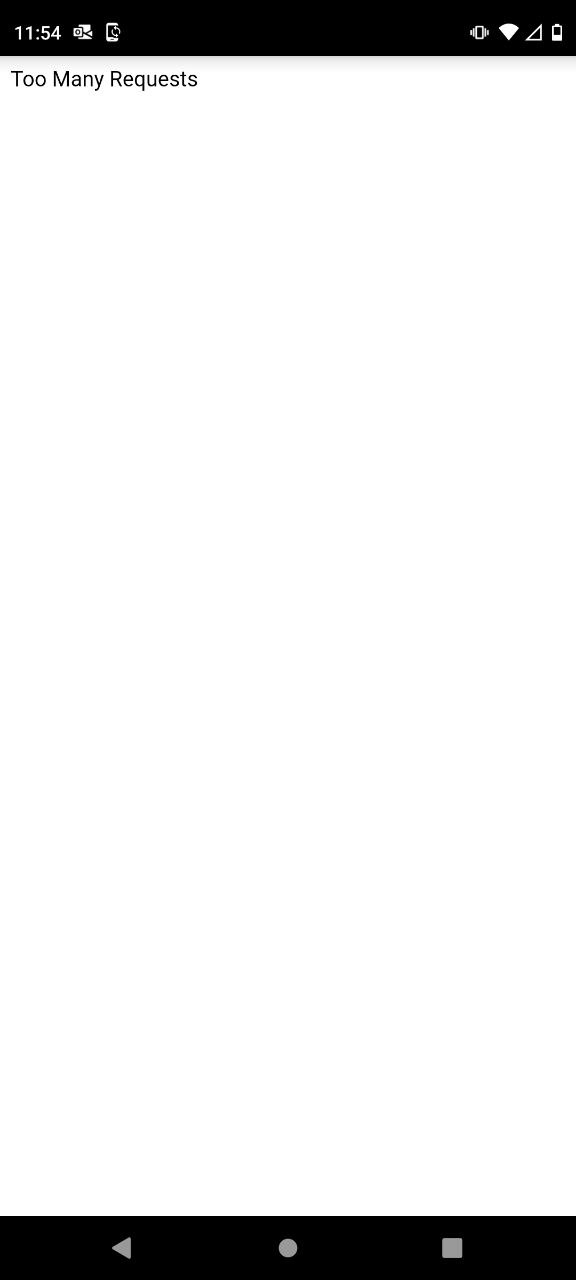
\includegraphics[width=0.3\textwidth]{./assets/microsoft_error_1.jpg}
  \caption{Erro de comunicação entre do aplicativo Microsoft Autenticator}
  \label{fig:MicrosoftAutenticatorErrorToManyReequests}
\end{figure}

Outro erro ocorreu ao tentar configurar uma outra conta de usuário que já utilizava o
duplo fator de autentiação para utilizar os recursos extras de autenticação, fucionando
de uma forma diferente, onde durante um processo de autenticação, será solicitado uma
confirmação de notificação no smartfone.
A aplicativo recebeu instruções para ativar o Bluetooth, embora atipico para esse tipo
de autentiação, ao tentar efetuar a autenticação, o aplicativo não respondeu e em tentativas
posteriores, ocorria erro no aplicativo.
No final, houve transtornos para recuperar o acesso a conta de usuário, pois nem mesmo os
metodos extras de autenticação funcionaram.

\begin{figure}[h!]
  \centering
  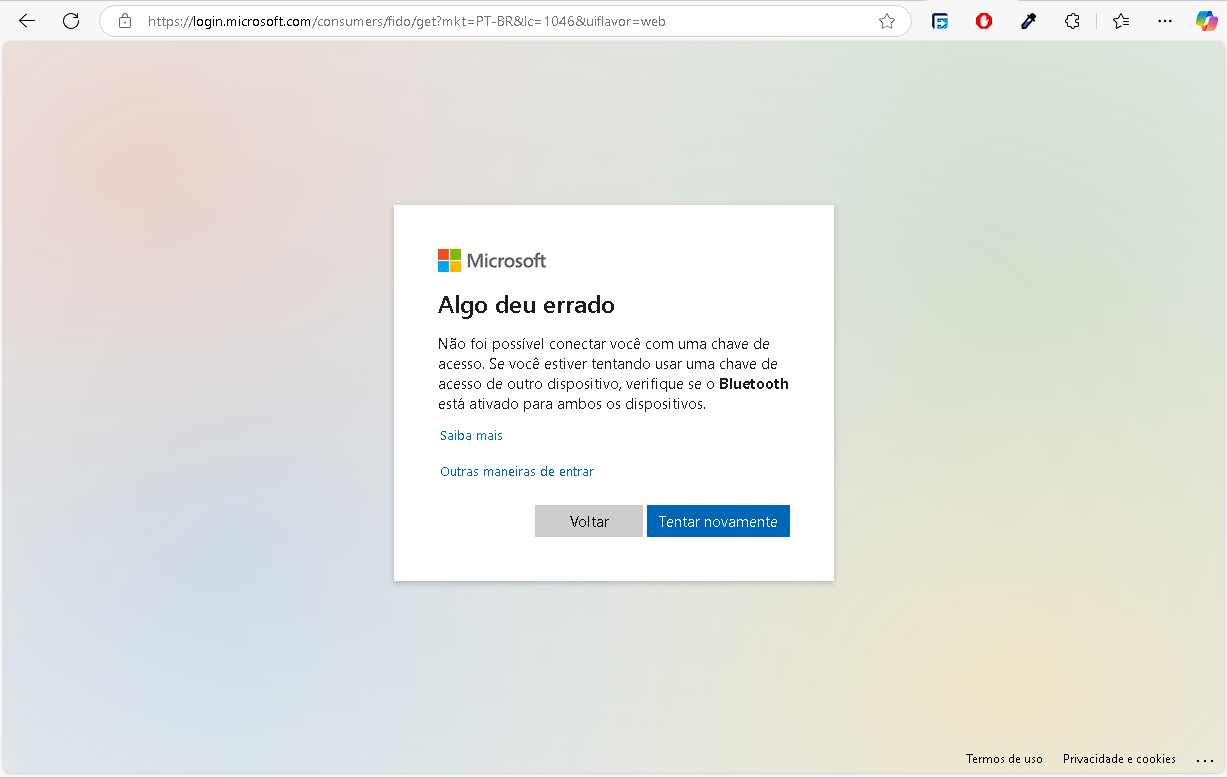
\includegraphics[width=0.7\textwidth]{./assets/microsoft_error_2.png}
  \caption{Erro no duplo fator de autentiação da Microsoft}
  \label{fig:Microsoft2FactoryAutenticatorError}
\end{figure}

\subsubsection{Aegis}

Já o Aegis, por ser um aplicativo de código aberto, oferece maior transparência
e controle sobre os dados do usuário, mas possui uma interface de configuração
e arquivos que pode ser menos amigável para usuários mais leigos.
Nele é possível adicionar e gerenciar chaves de autentiação de dois fatos,
exportar e importar cópias de segurançats para diversos aplicativos ou em formato de arquivos,
inclusive em formato criptografado.

A maior vantagem do Aegis é a possibilidade de instalar o aplicativo por meio da
loja de aplicativos de código aberto F-Droid, uma alternativa ao Google Play
Store, permitindo que o mesmo possa ser intalado em dispositivos Android sem GMS
ou AOSP (Android Open Source Project).

\subsection{Avaliação de Aplicativos de Gerenciamento de Senhas}

No sistema operacional Android com GMS o Google automaticamente oferece um popup
para salvar a senha no momento em que é digitada no processo de autenticação de
algum aplicativo ou serviço.
Como o Google não é especificamente um aplicativo de segurança, pode parecer um
pouco escondido a opção de gerenciar as senhas pelas configurações de conta.
Além do gerenciamento de senhas com sincronização em nuvem, é possível adicionar
anotações, exportar e importar em formato de plianilha CSV sem criptografia.

O mesmo pop-up do Android utilizado pelo Google pode ser substituido por
aplicativos de terceiros, como o Microsoft Authenticator, citado anteriormente
que oferece recursos adicionais para gerenciar senhas.
Também permite adicionar anotações, exportar e importar em formato de plianilha
CSV sem criptografia.

No sistema operacional Windows não há opção nativa ou pré instalada para
salvar senhas, dependendo de programas de terceiros para salvar senhas.
Navegadores de internet normalmente oferecem uma opção nativa para salvar senhas,
mas com poucos recursos extras de segurança ou gerenciamento.
Infelismente os navegadores de internet não solicitam uma senha mestre para liberar
a autenticação ou até mesmo para visualizar a senha.

\subsubsection{KeePass}

O KeePass é um aplicativo ou programa de código aberto para computadores pessoais.
Diferente dos aplicativos citados anteriormente, o KeePass não é um aplicativo
para dispositivos móveis como tablets ou smartfone, mas sim um aplicativo desktop,
que pode ser instalado em qualquer dispositivo com sistema operacional Windows.
Existem também versões para outros sistemas operacionais como Linux, Mac OS e até
BSD, desenvolvido por contribuidores não oficiais.

Por padrão o KeePass é em inglês, necessitando de plugins de tradução para outras
idiomas.
Embora a interface aparente ser para computadores mais antigos, não se trata de um
aplicativo desatualizado, mas sim um aplicativo com uma interface única, compatível
com qualquer sistema operacional recente.
Além de que a interface é amigável para gerenciar senhas, com maior foco no gerenciamento
das anotações e com sugestões inteligentes de senhas fortes.
Porém, sem integração com o sistema operacional, ou seja, nele, o usuário vai apenas
realizar anotações, sem possibilidade de auto completar senhas em processos de autentiação
e sem sincronização com outros dispositivos.

O KeePass permite salvar as senhas em formato de arquivos com criptografia, os arquivos
são salvos localmente pelo qual o usuário deve se compromenter em salvar em um local
seguro e manter cópias de segurança em outros locais.
Entretanto, o próprio aplicativo oferece e sugere a possibilidade de imprimir uma cópia
de segurança do arquivo de senhas.

\subsubsection{KeeWeb}

No site oficial de KeePass exístem vários aplicativos que são contribuições não oficiais
de KeePass, como KeeWeb que é um aplicativo de código aberto compatível com KeePass, em
que é possível utilizar o mesmo banco de dados do KeePass.
Diferente dos aplicativos citados anteriormente, o KeeWeb não é um aplicativo
nativo, mas sim um aplicativo web progressivo, multi plataforma, que pode ser instalado
em qualquer dispositivo com navegador de internet.
Assim como KeePass, não há integração com o sistema operacional para auto completar senhas
em processo de autenticação.

Por padrão o KeeWeb é em inglês, também necessitando de plugins de tradução para outros
idiomas, porém com a praticidade de poder instalar os plugins diretamente pelo aplicativo.
O KeeWeb apresenta uma interface moderna e amigável para gerenciar senhas, com o mesmo foco
no gerenciamento das anotações assim como no KeePass.

O KeeWeb permite salvar as anotações de senhas com ou sem criptografia, os arquivos ficam
dentro da memoria do navegador de internet e podem ser exportados localmente em formato de
arquivos.
Há um diferencial nesse aplicativo que permite exportar os arquivos em nuvens de serviços
de terceiros em que o usuários tiver preferencia.

Utilizar aplicativos de gerenciamento de senhas, apresentou grande praticidade,
especialmente para os serviços que não se mantem autenticados, solicitam a
autenticação com frequencia ou perdem a autenticação por defeito.
Porém os aplicativos de gerenciamento de senhas e navegadores de internet não
são perfeitos, em alguns casos, apresnetam o popup sob a caixa de entrada do
login, senha ou botões.
Já o KeeWeb, quando não configurado para o mesmo idioma do dispositivo, é
prejudicado no sistema operacional Android, por ser um aplicativo web progressivo,
o Google Chrome insiste em traduzir o aplicativo e até mesmo as senhas, tornando
as senhas inválidas.

\section{Considerações Finais}

A pesquisa revelou que mais da metade dos participantes possuem um nível de
conscientização sobre a importância da segurança digital, demonstrado pelo uso de
senhas fortes e pela autenticação de dois fatores.
No entanto, algumas práticas de segurança do restante dos participantes, como senhas
fracas e permanecer autenticado, ainda podem ser melhoradas.

Uma parcela significativa dos participantes já teve problemas de segurança, o que
indica que as práticas atuais não são totalmente eficazes.
A pontuação média da segurança em serviços digitais e da segurança pessoal indica
espaço para melhorias das ações pessoais e dos serviços digitais.

O duplo fator de autenticação é uma camada adicional de segurança que pode proteger
as contas dos usuários.
No entanto, essa tecnologia só está disponível para dispositivos móveis, além das
chaves físicas, sendo indispensável que todos os usuários realizem cópias de sergurança
para evitar complicações.

Embora existam aplicativos e programas variados de segurança pessoal, não é tão simples
de escolher o aplicativos ou programa mais adequando para o uso pessoal já que a
complexidade tecnica é um obstáculo.
Experimentar cada aplicativo ou programa para encontrar o mais adequado exige muito tempo
e organização.
Especialmente se tratando de aplicativos ou programas para anotar senhas, há poucas
opções de referências, ainda mais com a transparência dos sistemas operacionais e
navegadores de internet com opções nativas ou pré instaladas, normalmente com pouco
recursos de segurança e gerenciamento.

Todo o serviço que é bem feito, vai usar um algoritmo de derivação de chave e
nunca vai salvar as senhas das credênciais de forma aberta.
Logo, se o mesmo limita o comprimento ou variabilidade de caracteres do cadastro da
senha, é um grande indicativo de que o serviço não está preocupado com a segurança
dos dados dos usuários.

Por mais sofisticados que os serviços digitais possam ser, não existe garantias de segurança.
Cada estratégia de segurança é uma camada a mais, uma barreira adicionado contra ataques.
Ao mesmo tempo, cada camada adiciona complexidade, necessitando de anotações, cópias de
segurança e até aplicativos confiaveis, do contrário, as camadas de segurança que deviam
proteger o usuário, pode se tornar um obstáculo para o próprio usuário.

A conscientização sobre esses golpes é crucial, pois o conhecimento é a
primeira linha de defesa contra os ataques cibernéticos.
É importante estar atento a mensagens suspeitas que solicitam dados
confidenciais ou contêm links e anexos desconhecidos. Para se proteger,
verifique a autenticidade das mensagens, não clique em links ou baixe
anexos de fontes desconhecidas e use soluções de segurança confiáveis.
Se receber um código de autenticação sem solicitar, não o informe a
ninguém e altere sua senha, pois pode ser uma tentativa de invasão.

\subsection{Anotações de Credênciais}

É improvável que uma pessoa possa memorizar muitas credênciais de acesso, especialmente com
alta entropia de senhas.
Optar por anotar as informações em um caderno requer menos desafios de informatização, porém
é mais trabalhoso e necessita de atenção ao representar caracteres especiais, letras
maiúsculas ou minúsculas para evitar erros.
Enquanto que anotar as informações em formato digital é mais fácil, mas requer conhecimento
de informatização, uso de programas ou aplicativos de terceiros e cuidado com o armazenamento
do arquivo.

Os principais navegadores de internet oferecem recursos simples para armazenar informações
básicas das credênciais de acesso, alguns até com a possibilidade de sincronizar as informações
entre dispositivos.
Por outro lado, para se ter mais controle de informações e recursos de seguraça, existem
programas e aplicativos de terceiros, oferecendo diversas vantagens.

De qualquer forma, deve-se evitar anotar senhas em lugares inapropriados como aplicativos de
bloco de notas, aplicativos de mensagens em geral ou até em formato de contatos de telefones,
pois todos esses recursos não são criptografados e normalmente não são projetados para esses
fins e podem ser explorados por usuários mal intencionados ou vulnerabilidades de segurança.

\bibliographystyle{sbc}
\bibliography{references}

\end{document}